\nonstopmode
\documentclass[aspectratio=169]{beamer}
\usepackage[utf8]{inputenc}
% \usepackage[frenchb]{babel}
\usepackage{amsmath}
\usepackage{mathtools}
\usepackage{breqn}
\usepackage{multirow}
\usetheme{boxes}
\usepackage{graphicx}
\usepackage{import}
\usepackage{adjustbox}
%\useoutertheme[footline=authortitle,subsection=false]{miniframes}
%\useoutertheme[footline=authorinstitute,subsection=false]{miniframes}
\useoutertheme{infolines}
\setbeamertemplate{headline}{}

\beamertemplatenavigationsymbolsempty

\definecolor{TitleOrange}{RGB}{255,137,0}
\setbeamercolor{title}{fg=TitleOrange}
\setbeamercolor{frametitle}{fg=TitleOrange}

\definecolor{ListOrange}{RGB}{255,145,5}
\setbeamertemplate{itemize item}{\color{ListOrange}$\blacktriangleright$}

\definecolor{verygrey}{RGB}{70,70,70}
\setbeamercolor{normal text}{fg=verygrey}


\usepackage{tabu}
\usepackage{multicol}
\usepackage{vwcol}
\usepackage{stmaryrd}
\usepackage{graphicx}

\usepackage[normalem]{ulem}

\AtBeginSection[]{
  \begin{frame}
  \vfill
  \centering
  \begin{beamercolorbox}[sep=8pt,center,shadow=true,rounded=true]{title}
    \usebeamerfont{title}\insertsectionhead\par%
  \end{beamercolorbox}
  \vfill
  \end{frame}
}

\title{Garage}
\subtitle{a lightweight and robust geo-distributed data storage system}
\author{Alex Auvolat, Deuxfleurs}
\date{SEED webinar, 2024-01-12}

\begin{document}

% \begin{frame}
% 	\centering
% 	
\includegraphics[width=.3\linewidth]{../../sticker/Garage.png}
% 	\vspace{1em}
% 
% 	{\large\bf Alex Auvolat, Deuxfleurs Association}
% 	\vspace{1em}
% 
% 	\url{https://garagehq.deuxfleurs.fr/}
% 
% 	%Matrix channel: \texttt{\#garage:deuxfleurs.fr}
% \end{frame}

\begin{frame}
	%\frametitle{Who I am}
	\begin{columns}[t]
		\begin{column}{.2\textwidth}
			\centering
			\adjincludegraphics[width=.4\linewidth, valign=t]{assets/alex.jpg}
		\end{column}
		\begin{column}{.6\textwidth}
			\textbf{Alex Auvolat}\\
			Member of Deuxfleurs, lead developer of Garage
		\end{column}
		\begin{column}{.2\textwidth}
			~
		\end{column}
	\end{columns}
	\vspace{.5em}

	\begin{columns}[t]
		\begin{column}{.2\textwidth}
			\centering
			\adjincludegraphics[width=.6\linewidth, valign=t]{../../logo/garage-notext.png}
		\end{column}
		\begin{column}{.6\textwidth}
			\\\textbf{Garage}\\
			A self-hosted alternative to S3 for object storage
		\end{column}
		\begin{column}{.2\textwidth}
			~
		\end{column}
	\end{columns}
	\vspace{2em}

	\begin{columns}[t]
		\begin{column}{.2\textwidth}
			\centering
			\adjincludegraphics[width=.5\linewidth, valign=t]{assets/deuxfleurs.pdf}
		\end{column}
		\begin{column}{.6\textwidth}
			\textbf{Deuxfleurs}\\
			A non-profit self-hosting collective,\\
			member of the CHATONS network
		\end{column}
		\begin{column}{.2\textwidth}
			\centering
			\adjincludegraphics[width=.7\linewidth, valign=t]{assets/logo_chatons.png}
		\end{column}
	\end{columns}

\end{frame}

\begin{frame}
	\frametitle{Stable vs Resilient}

	\hspace{1em}
	\begin{minipage}{7cm}
		\textbf{Building a "stable" system:}
		\vspace{1em}

		Enterprise-grade systems typically employ:
		\vspace{1em}
		\begin{itemize}
			\item RAID
			\item Redundant power grid + UPS
			\item Redundant Internet connections
			\item Low-latency links
			\item ... 
		\end{itemize}
		\vspace{1em}
		$\to$ costly, only worth at DC scale\\
		$\to$ still risk of DC-level incident...
	\end{minipage}
	\hfill
	\begin{minipage}{7cm}
		\textbf{Building a \underline{resilient} system:}
		\vspace{1em}

		An alternative, cheaper way:
		\vspace{1em}
		\begin{itemize}
			\item Commodity hardware \\(e.g. old desktop PCs)
				\vspace{.5em}
			\item Commodity Internet \\(e.g. FTTB, FTTH) and power grid
				\vspace{.5em}
			\item \textbf{Geographical redundancy} \\(multi-site replication)
		\end{itemize}
		\vspace{1.5em}
	\end{minipage}
	\hspace{1em}
\end{frame}

\begin{frame}
	\frametitle{Example: our infrastructure at Deuxfleurs}
	\only<1>{
		\begin{center}
			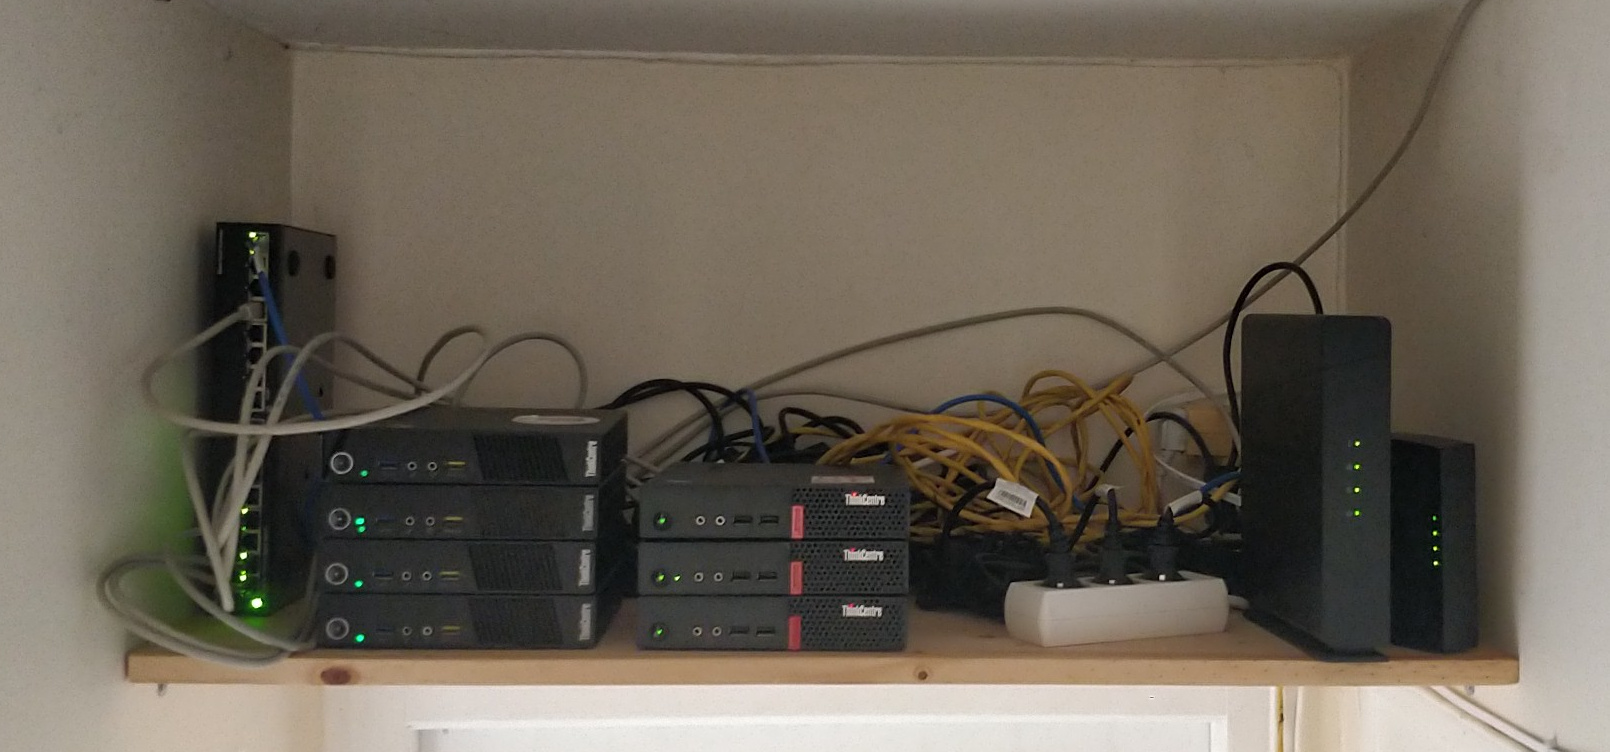
\includegraphics[width=.8\linewidth]{assets/neptune.jpg}
		\end{center}
	}
	\only<2>{
		\begin{center}
			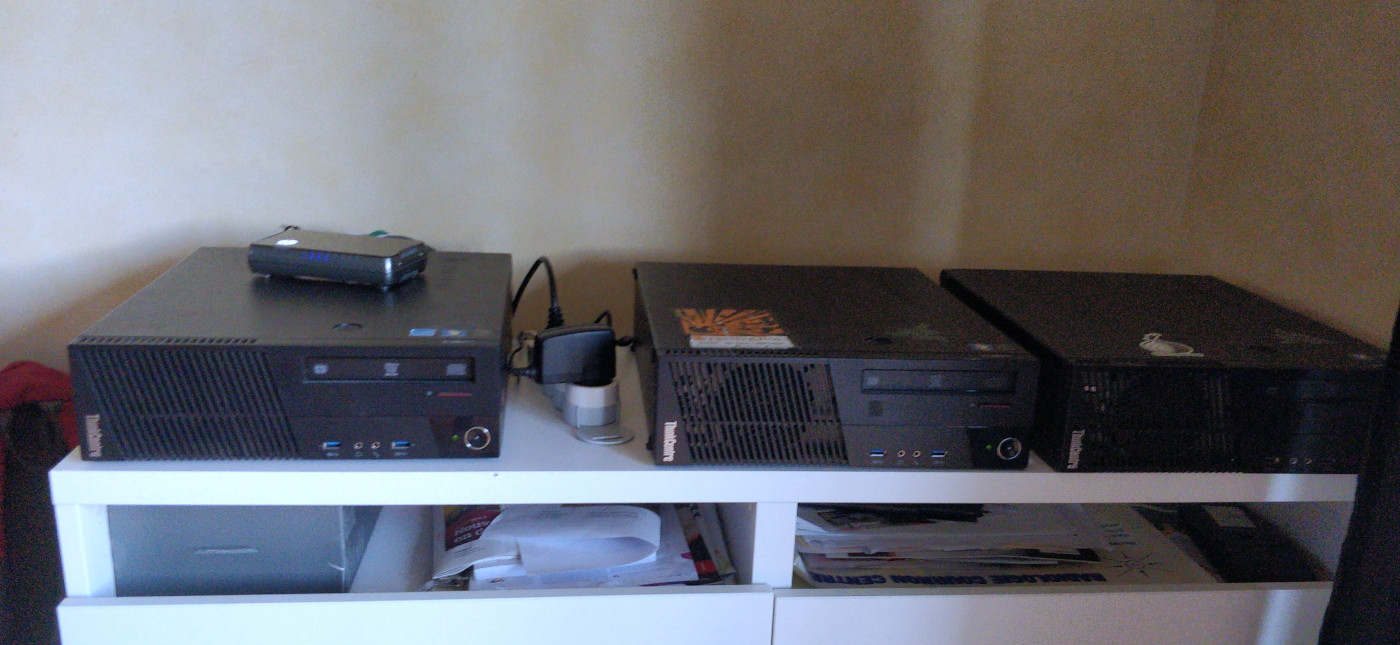
\includegraphics[width=.8\linewidth]{assets/atuin.jpg}
		\end{center}
	}
	\only<3>{
		\begin{center}
			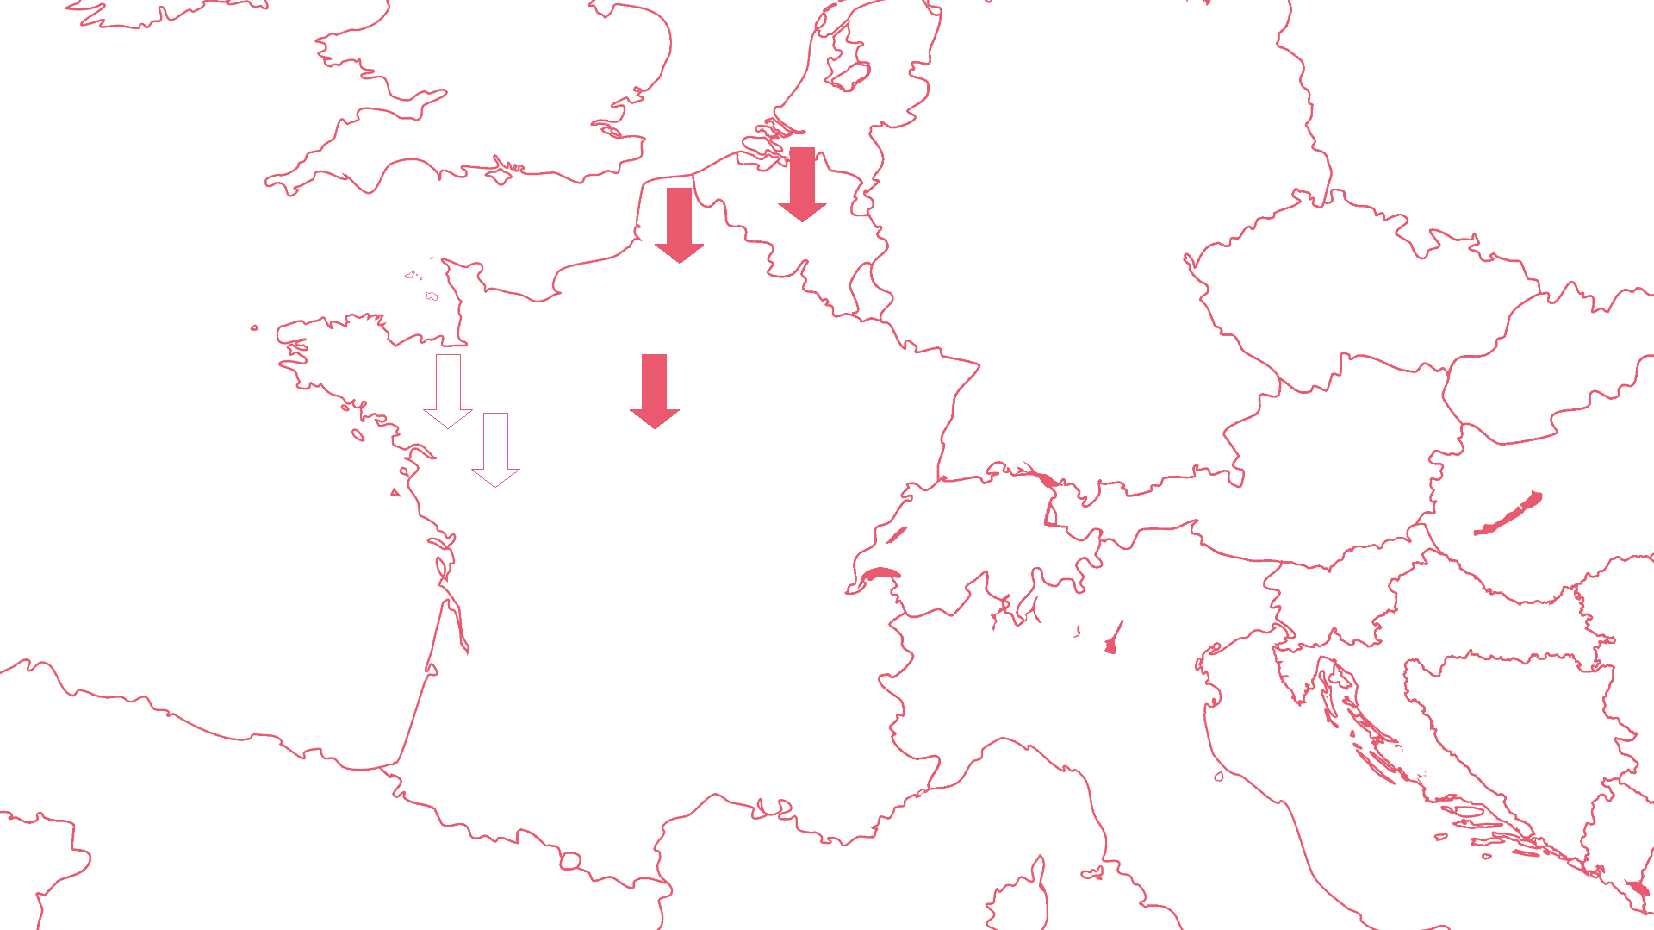
\includegraphics[width=.8\linewidth]{assets/inframap_jdll2023.pdf}
		\end{center}
	}
\end{frame}

\begin{frame}
	\frametitle{Object storage: simpler than file systems}

	\begin{minipage}{6cm}
		Only two operations:
		\vspace{1em}
		\begin{itemize}
			\item Put an object at a key
				\vspace{1em}
			\item Retrieve an object from its key
		\end{itemize}
		\vspace{1em}
		{\footnotesize (and a few others)}

		\vspace{1em}
		Sufficient for many applications!
	\end{minipage}
	\hfill
	\begin{minipage}{8cm}
		\begin{center}
			\vspace{2em}
			
\includegraphics[height=6em]{../2020-12-02_wide-team/img/Amazon-S3.jpg}
			\hspace{2em}
			
\includegraphics[height=5em]{assets/minio.png}

			\vspace{2em}
			
\includegraphics[height=6em]{../../logo/garage_hires_crop.png}
		\end{center}
		\vspace{1em}
	\end{minipage}
\end{frame}


\begin{frame}
	\frametitle{The data model of object storage}
	Object storage is basically a key-value store:
	\vspace{1em}

		\begin{center}
		\begin{tabular}{|l|p{8cm}|}
			\hline
			\textbf{Key: file path + name} & \textbf{Value: file data + metadata} \\
			\hline
			\hline
			\texttt{index.html} &
				\texttt{Content-Type: text/html; charset=utf-8} \newline
				\texttt{Content-Length: 24929} \newline
				\texttt{<binary blob>} \\ 
			\hline
			\texttt{img/logo.svg} &
				\texttt{Content-Type: text/svg+xml} \newline
				\texttt{Content-Length: 13429} \newline
				\texttt{<binary blob>} \\ 
			\hline
			\texttt{download/index.html} &
				\texttt{Content-Type: text/html; charset=utf-8} \newline
				\texttt{Content-Length: 26563} \newline
				\texttt{<binary blob>} \\ 
			\hline
		\end{tabular}
		\end{center}
\end{frame}

\begin{frame}
	\frametitle{Implementation: consensus vs weak consistency}

	\hspace{1em}
	\begin{minipage}{7cm}
		\textbf{Consensus-based systems:}
		\vspace{1em}
		\begin{itemize}
			\item \textbf{Leader-based:} a leader is elected to coordinate
				all reads and writes
				\vspace{1em}
			\item Allows for \textbf{sequential reasoning}:
				program as if running on a single machine
				\vspace{1em}
			\item Serializability is one of the \\
				\textbf{strongest consistency guarantees}
				\vspace{1em}
			\item \textbf{Costly}, the leader is a bottleneck;
				leader elections on failure take time
		\end{itemize}
	\end{minipage}
	\hfill
	\begin{minipage}{7cm} \visible<2->{
		\textbf{Weakly consistent systems:}
		\vspace{1em}
		\begin{itemize}
			\item \textbf{Nodes are equivalent}, any node
				can originate a read or write operation
				\vspace{1em}
			\item \textbf{Operations must be independent},
				conflicts are resolved after the fact
				\vspace{1em}
			\item Strongest achievable consistency:\\
				\textbf{read-after-write consistency}\\(using quorums)
				\vspace{1em}
			\item \textbf{Fast}, no single bottleneck;\\
				works transparently with offline nodes
		\end{itemize}
	} \end{minipage}
	\hspace{1em}
\end{frame}

\begin{frame}
	\frametitle{Why avoid consensus?}
	Consensus can be implemented reasonably well in practice, so why avoid it?
	\vspace{2em}
	\begin{itemize}
		\item \textbf{Software complexity:} RAFT and PAXOS are complex beasts;\\
			harder to prove, harder to reason about
			\vspace{1.5em}
		\item \textbf{Performance issues:}
			\vspace{1em}
			\begin{itemize}
				\item Taking a decision may take an \textbf{arbitrary number of steps} (in adverse scenarios)
					\vspace{1em}
				\item The leader is a \textbf{bottleneck} for all requests;\\
					even in leaderless approaches, \textbf{all nodes must process all operations in order}
					\vspace{1em}
				\item Particularly \textbf{sensitive to higher latency} between nodes
			\end{itemize}
	\end{itemize}
\end{frame}

\begin{frame}
	\frametitle{Objective: the right level of consistency for Garage}

	\underline{Constraints:} slow network (geographical distance), node unavailability/crashes\\
	\underline{Objective:} maximize availability, maintain an \emph{appropriate level of consistency}\\
	\vspace{1em}
	\begin{enumerate}
		\item<2-> \textbf{Weak consistency for most things}\\
			\vspace{1em}
			\underline{Example:} \texttt{PutObject}\\
			\vspace{.5em}
			If two clients write the same
			object at the same time, one of the two is implicitly overwritten.
			No need to coordinate, use a \emph{last-writer-wins register}.
			\vspace{1em}
		\item<3-> \textbf{Stronger consistency only when necessary}\\
			\vspace{1em}
			\underline{Example:} \texttt{CreateBucket}\\
			\vspace{.5em}
			A bucket is a reserved name in a shared namespace,
			two clients should be prevented from both creating the same bucket
			(\emph{mutual exclusion}).
	\end{enumerate}
\end{frame}

\begin{frame}
	\frametitle{The possibility of \emph{leaderless consensus}}
	Currently, Garage \emph{only has weak consistency}. Is fast, but \texttt{CreateBucket} is broken!

	\visible<2->{
		\vspace{1em}
		Leaderless consensus (Antoniadis et al., 2023) alleviates issues with RAFT and PAXOS:
			\vspace{1em}
		\begin{itemize}
			\item \textbf{No leader.} All nodes participate equally at each time step,
				and different nodes can be unavailable at different times without issues.
				\\ \vspace{.5em} $\to$ better tolerance to the high latency (remove bottleneck issue)
				\\ $\to$ tolerates crash transparently
				\vspace{1em}
			\item \textbf{Simpler formalization.} The algorithm is very simple to express and to analyze in mathematical terms.
		\end{itemize}
	}
	\visible<3->{
		\vspace{1em}
		One of the possible subjects for this PhD:
		\\$\to$ \emph{integration of leaderless consensus in Garage} + testing + perf eval, etc.
	}
\end{frame}

\begin{frame}
	\begin{center}
			\includegraphics[width=.25\linewidth]{../../logo/garage_hires.png}\\
			\vspace{-1em}
		\url{https://garagehq.deuxfleurs.fr/}\\
		\url{mailto:garagehq@deuxfleurs.fr}\\
		\texttt{\#garage:deuxfleurs.fr} on Matrix

		\vspace{1.5em}
			
\includegraphics[width=.06\linewidth]{assets/rust_logo.png}
			
\includegraphics[width=.13\linewidth]{assets/AGPLv3_Logo.png}
	\end{center}
\end{frame}

\end{document}

%% vim: set ts=4 sw=4 tw=0 noet spelllang=en :
